\documentclass[reprint, nofootinbib, nobalancelastpage, 10pt]{revtex4-2}

\usepackage[T2A]{fontenc}			% кодировка
\usepackage[utf8]{inputenc}			% кодировка исходного текста
\usepackage[english,russian]{babel}	% локализация и переносы

\usepackage{amsmath,amsfonts,amssymb,amsthm,mathtools}

\usepackage[usenames]{color}
\usepackage{colortbl}
\usepackage{indentfirst} %Красная строка
\usepackage{hyperref}

\usepackage{booktabs}
\usepackage{graphicx}  % Для вставки рисунков
\graphicspath{{images/}{graphs/}}  % папки с картинками

\renewcommand*{\thefootnote}{\alph{footnote}}

\begin{document}

\title{Исследование эффекта Комптона}
\author{Илларионов Владислав}
\affiliation{группа Б04-855}

\maketitle


\section*{Введение}

С помощью сцинтилляционного спектрометра исследуется энергетический спектр
$\gamma$-квантов, рассеянных на графите. Определяется энергия рассеянных
\mbox{$\gamma$-квантов} в зависимости от угла рассеяния, а также энергия покоя частиц,
на которых происходит комптоновское рассеяние.


\section*{Теоретическая часть}

Эффект Комптона -- увеличение длины волны рассеянного излучения по сравнению с падающим --
интерпретируется как результат упругого соударения фотона и свободного электрона.

Изменение длины волны равно:
\begin{equation}
	\label{eq:kompton_lmbs}
	\Delta \lambda = \lambda_1 - \lambda_0 = \dfrac{h}{mc}(1 - \cos \theta) =
		\Lambda_{\text{к}} (1 - \cos \theta),
\end{equation}
где $\lambda_0$ и $\lambda_1$ -- длины волн фотона до и после рассеяния на угол $\theta$,
а $\Lambda_{\text{к}} = 2.42 \cdot 10^{-10}$ см -- комптоновская длина волны электрона.

Преобразуем формулу~(\ref*{eq:kompton_lmbs}), перейдя от длин волн к энергиям фотонов:
\begin{equation}
	\label{eq:kompton_enrg}
	\dfrac{1}{\varepsilon(\theta)} - \dfrac{1}{\varepsilon_0} = 1 - \cos \theta
\end{equation}

Здесь $\varepsilon_0 = E_0/(mc^2)$ -- выраженная в единицах $mc^2$ энергия фотонов,
падающих на рассеиватель, $\varepsilon(\theta)$ -- выраженная в тех же единицах энергия
квантов, испытавших комптоновское рассеяние на угол $\theta$, m -- масса электрона.


\section*{Экспериментальная установка}


Блок-схема установки изображена на рисунке \ref{img:pic1}.\\ Источником излучения 1 служит
$^{137}$Cs, испускающий $\gamma$-лучи с энергией 662 кэВ. Он помещен в толстостенный
свинцовый контейнер с коллиматором. Сформированный коллиматором узкий пучок
$\gamma$-квантов попадает на графитовую мишень 2 (цилиндр диаметром 40 мм и высотой 100 мм).

Кванты, испытавшие комптоновское рассеяние в мишени, регистрируются сцинтилляционным
счетчиком. Счетчик состоит из фотоэлектронного умножителя 3 (далее ФЭУ) и сцинтиллятора 4.
Сцинтиллятором служит кристалл NaI(Ti) цилиндрической формы диаметром 40 мм и
высотой 40 мм, его выходное окно находится в оптическом контакте с фотокатодом ФЭУ.
Сигналы возникающие на аноде ФЭУ, подаются на ЭВМ для амплитудного анализа. Кристалл и ФЭУ
расположены в светонепроницаемом блоке, укрепленном на горизонтальной штанге. Штанга
вместе с этим блоком может вращаться относительно мишени, угол поворота рассчитывается по
лимбу 6.

Головная часть сцинтилляционного блока закрыта свинцовым коллиматором 5, который формирует
входной пучок и защищает детектор от постороннего излучения.

\begin{figure}[h!]	\caption{Результаты измерений}
	\label{tab:data}
	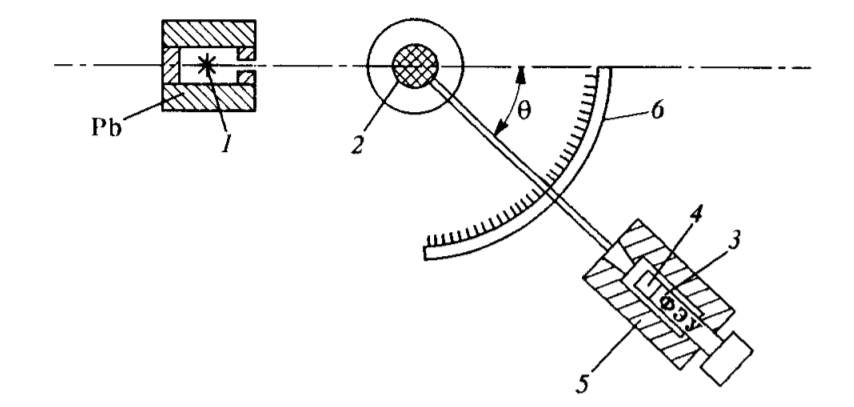
\includegraphics[width = \linewidth]{pic1.png}
	\caption{Блок-схема установки по изучению рассеяния $\gamma$-квантов}
	\label{img:pic1}
\end{figure}

На рисунке \ref{img:pic2} представлена функциональная блок-схема измерительного комплекса,
который состоит из ФЭУ, питаемого от высоковольтного выпрямителя ВСВ,
усилителя-анализатора УА, являющегося входным интерфейсом ЭВМ, управляемой с клавиатуры КЛ.
В ходе проведения эксперимента информация отображается на экране дисплея Д.

\begin{figure}[h!]
	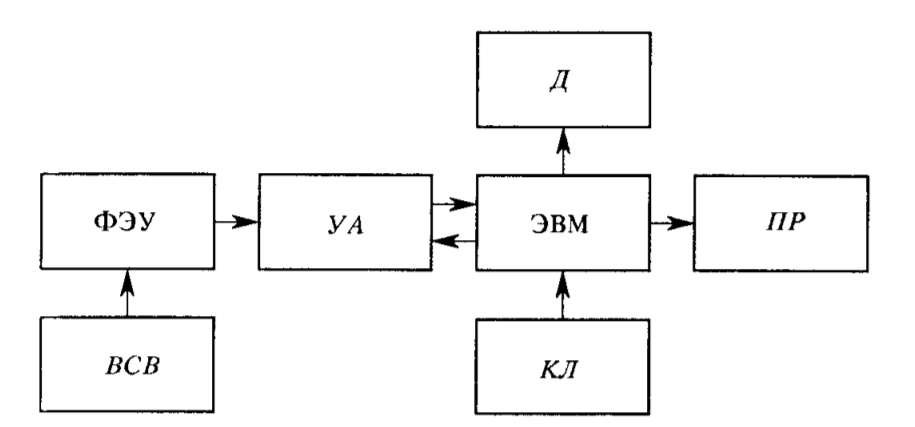
\includegraphics[width = \linewidth]{pic2.png}
	\caption{Блок-схема измерительного комплекса}
	\label{img:pic2}
\end{figure}

Под действием монохроматического излучения на выходе ФЭУ возникает распределение
электрических импульсов (рис. \ref{img:pic3}). В амплитудном распределении импульсов
имеется так называемый фотопик, возникающий в результате фотоэффекта, и обязанное
комптоновскому рассеянию сплошное распределение. Положение фотопика однозначно связано с
энергией регистрируемого $\gamma$-излучения. Соответственно нас будет интересовать
положение (номер канала) вершины этого пика в зависимости от угла поворота детектора.

\begin{figure}[h!]
	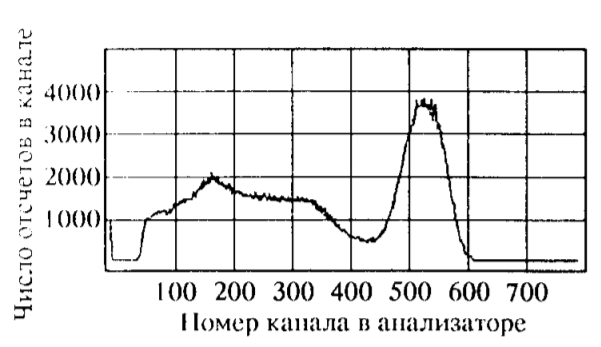
\includegraphics[width = \linewidth]{pic3.png}
	\caption{Амплитудное распределение импульсов, возникающих
		под действием монохроматических $\gamma$-квантов в сцинтилляторе NaI(Ti)}
	\label{img:pic3}
\end{figure}


\section*{Методика измерения}

\begin{enumerate}
	\item Включим все измерительные устройства и компьютер
	\item Запустим программу и войдём режим измерения спектра
	\item Устанавливая сцинтилляционный счетчик под разными углами $\theta$ к первоначальному
		направлению полета фотонов и вводя значения этих углов в ЭВМ, снимем амплитудные
		спектры и определим положения фотопиков для каждого $\theta$; измерения проводим с
		шагом в $10^\circ$ в диапазоне от $0^\circ$ до $120^\circ$. Также учтем, что с
		увеличением угла интенсивность рассеянных фотонов уменьшается, поэтому будем
		увеличивать время проведения замера.
\end{enumerate}

Заменим в формуле~(\ref{eq:kompton_enrg}) $\varepsilon(\theta)$ номером канала $N(\theta)$,
соответствующего вершине фотопика в спектре для угла $\theta$. Обозначая буквой $A$
неизвестный коэффициент пропорциональности между $\varepsilon(\theta)$ и $N(\theta)$,
получим:
\begin{equation}
	\label{eq:kompton_n}
	\dfrac{1}{N(\theta)} - \dfrac{1}{N(0^\circ)} = A (1 - \cos \theta)
\end{equation}

Используя экспериментальные данные, построим график, откладывая по оси абсцисс величину
$1 - \cos \theta$, а по оси ординат величину $1/N(\theta)$. Согласно
формуле~(\ref{eq:kompton_n}) получится линейная зависимость.

Для аппроксимации будем использовать взвешенный МНК, минимизируем взвешенную сумму
квадратов остатков:
\[\text{WRSS} = \sum_{i=1}^n \left( \dfrac{\Delta y_i}{\sigma_i} \right)^2 \longrightarrow \min\]

Здесь $\Delta y_i = y_i - kx_i - b$, $\sigma_i$ -- погрешность определения $1/N(\theta)$.
Погрешность коэффициентов линейной модели определяется из оценки ковариационной матрицы. 

По полученной аппроксимации рассчитываются значения $N_{\text{наил}}(0^\circ)$,
$N_\text{наил}(90^\circ)$.

Возвращаясь от переменной $\varepsilon$ к энергии $E$, получаем, что при $\theta=90^\circ$,
формула~(\ref{eq:kompton_enrg}) принимает вид:
\[mc^2 \left( \dfrac{1}{E(90^\circ)} - \dfrac{1}{E(0^\circ)} \right) = 1\]

или:
\begin{equation}
	\label{eq:res}
	mc^2 = E_{\gamma} \dfrac{N(90^\circ)}{N(0^\circ) - N(90^\circ)}
\end{equation}
	

\section*{Обработка данных}

Проведём измерения описанные в предыдущем разделе и занесём результаты в
таблицу~\ref{tab:data}.

По полученным данным построим график зависимости $1/N(\theta)$ от $(1 - \cos \theta)$
(см.~рис.~\ref{graph:plot}). Аппроксимируем график прямой $y = kx + b$. Полученные
коэффициенты:
\begin{eqnarray*}
	k &= (167 \pm 7) \cdot 10^{-5}\\
	b &= (123 \pm 2) \cdot 10^{-5}
\end{eqnarray*}

\begin{figure}[h!]
	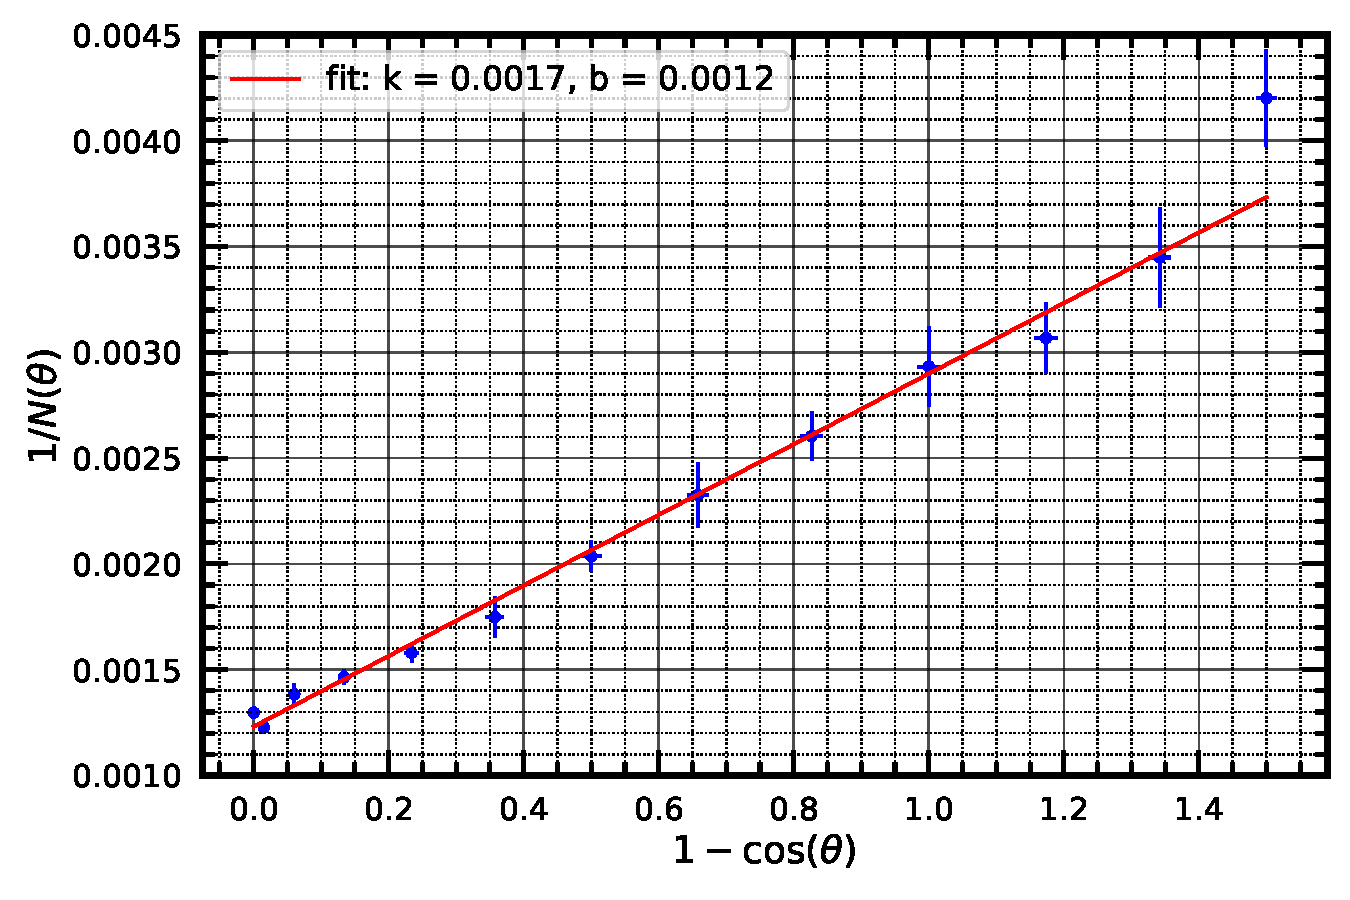
\includegraphics[width=\linewidth]{plot.pdf}
	\caption{График зависимости $1/N(\theta)$ от $(1 - \cos \theta)$}
	\label{graph:plot}
\end{figure}

Теперь можем найти $N_{\text{наил}}(0^\circ)$, $N_\text{наил}(90^\circ)$:
\begin{eqnarray*}
	&N_{\text{наил}}(0^\circ) &= 813 \pm 11\\
	&N_\text{наил}(90^\circ)  &= 345 \pm 9
\end{eqnarray*}

Из формулы~(\ref{eq:res}), учитывая, что $E_\gamma = 662$ кэВ, найдем энергию покоя
электрона:
\[mc^2 = 488 \pm 27 \text{ кэВ}\]


\section*{Вывод}

В ходе данной работы был исследован эффект Комптона. Была рассчитана энергия покоя
электрона $mc^2 = 488 \pm 27 \text{ кэВ}$, значение которой совпадает с табличным 511 кэВ
в пределах погрешности, что подтверждает справедливость квантового описания эффекта
Комптона.

Точность измерения составила 5.5\%. Основной вклад в погрешность вносят большие значения
для ширины фотопиков. Можно снизить эту погрешность, увеличив время измерений.


\appendix

\newpage
\section{Таблицы}

\begin{table}[h!]
	\caption{Результаты измерений}
	\label{tab:data}
	\begin{tabular}{lcccccc}
		\toprule
		$\theta$ & {} & N($\theta$) & {} &  $1/N(\theta) \cdot 10^3$ & {} &  $1 - \cos \theta$ \\
		\midrule
		$0^{\circ}$   & {} & 771 $\pm$ 18 & {} & 1.30 $\pm$ 0.03 & {} & 0     $\pm$ 0.0003\\
		$10^{\circ}$  & {} & 815 $\pm$ 13 & {} & 1.23 $\pm$ 0.02 & {} & 0.015 $\pm$ 0.003 \\
		$20^{\circ}$  & {} & 723 $\pm$ 26 & {} & 1.38 $\pm$ 0.05 & {} & 0.060 $\pm$ 0.006 \\
		$30^{\circ}$  & {} & 683 $\pm$ 16 & {} & 1.46 $\pm$ 0.03 & {} & 0.134 $\pm$ 0.009 \\
		$40^{\circ}$  & {} & 633 $\pm$ 19 & {} & 1.58 $\pm$ 0.05 & {} & 0.234 $\pm$ 0.011 \\
		$50^{\circ}$  & {} & 572 $\pm$ 32 & {} & 1.75 $\pm$ 0.10 & {} & 0.357 $\pm$ 0.013 \\
		$60^{\circ}$  & {} & 491 $\pm$ 18 & {} & 2.04 $\pm$ 0.07 & {} & 0.500 $\pm$ 0.015 \\
		$70^{\circ}$  & {} & 438 $\pm$ 28 & {} & 2.28 $\pm$ 0.15 & {} & 0.658 $\pm$ 0.016 \\
		$80^{\circ}$  & {} & 384 $\pm$ 17 & {} & 2.60 $\pm$ 0.12 & {} & 0.826 $\pm$ 0.017 \\
		$90^{\circ}$  & {} & 341 $\pm$ 22 & {} & 2.93 $\pm$ 0.19 & {} & 1.000 $\pm$ 0.017 \\
		$100^{\circ}$ & {} & 326 $\pm$ 18 & {} & 3.07 $\pm$ 0.17 & {} & 1.173 $\pm$ 0.017 \\
		$110^{\circ}$ & {} & 290 $\pm$ 20 & {} & 3.45 $\pm$ 0.24 & {} & 1.342 $\pm$ 0.016 \\
		$120^{\circ}$ & {} & 238 $\pm$ 13 & {} & 4.20 $\pm$ 0.23 & {} & 1.500 $\pm$ 0.015 \\
		\bottomrule
	\end{tabular}
\end{table}

\section{Иллюстрации}

\begin{figure}[h!]
	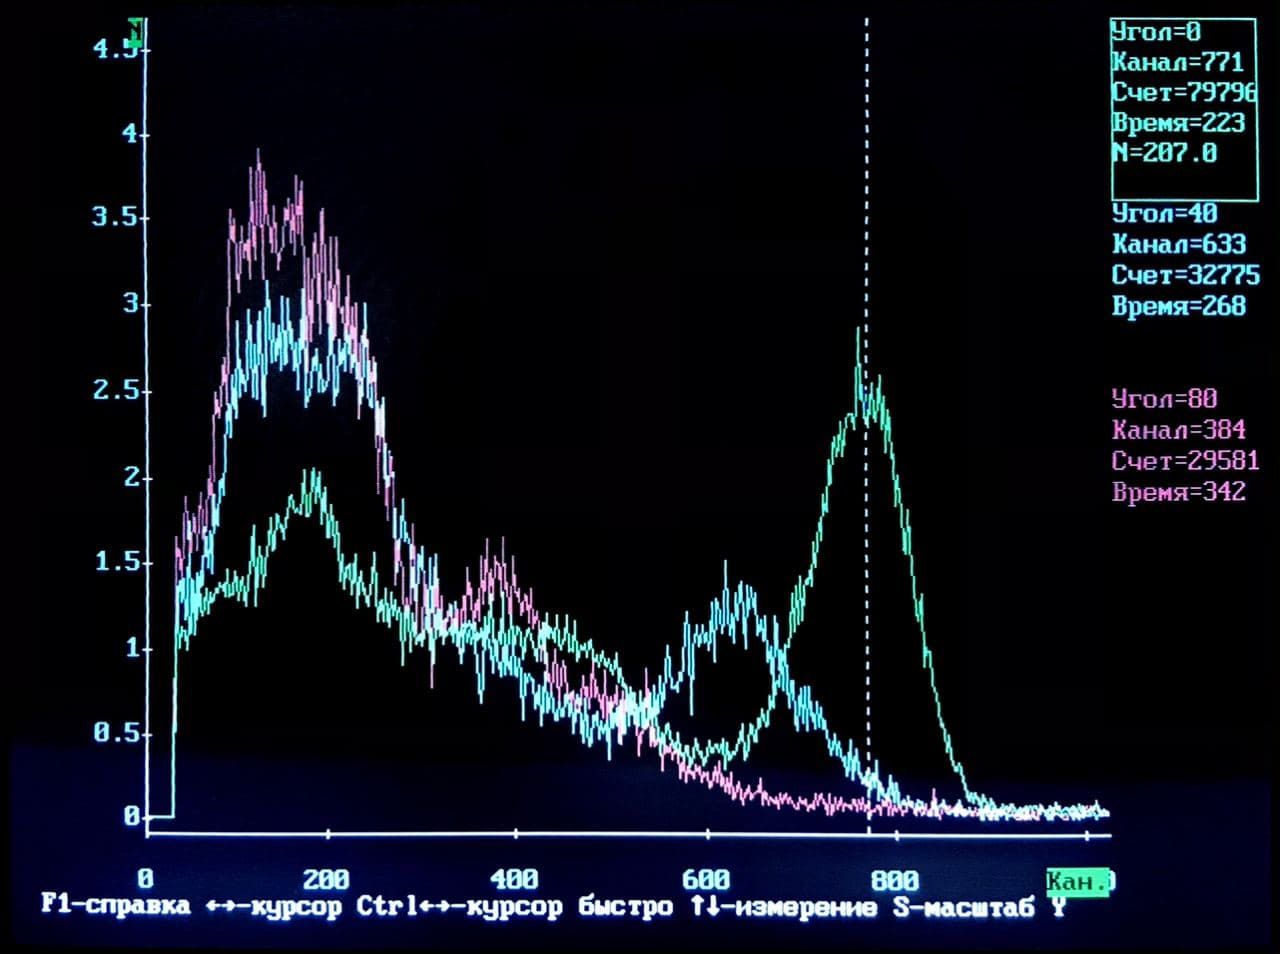
\includegraphics[width=\linewidth]{pic4.jpg}
	\caption{Амплитудное распределение импульсов для различных значений $\theta$}
	\label{img:pic4}
\end{figure}


\end{document}